\begin{figure}[h]
\centering
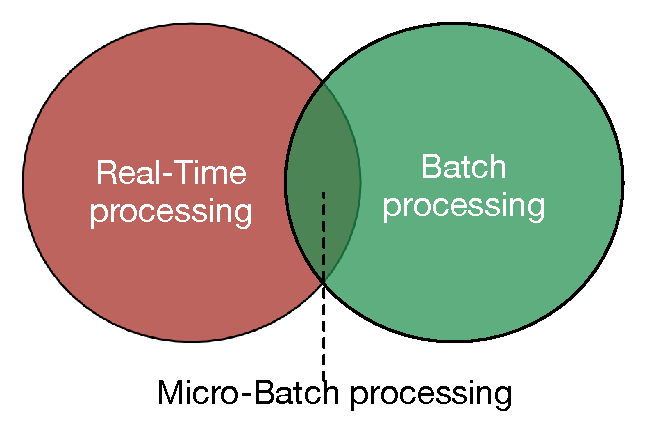
\includegraphics[width=0.6\textwidth]{eps/streambatch}
\caption{Conceptual view of micro-batching}
\label{fig_micro_batch}
\end{figure}







\section{Evaluation}
\label{eval}
\subsection{Configuration}
The following configurations are used throughput experiments:
\begin{itemize}
\item Cluster size: 2,3,4 and 8 node clusters
\item Parallelism within single node: number of cores, which is 16.
\item Parallelism within cluster: (Parallelism within single node) * (number of nodes)

\item Backpressure: enabled in all systems
\item Network bandwidth: 1Gb
\item Number of Data Engines running in parallel: 16
\item Allocated memory: 16GB
\item Cluster type: Standalone
\item Input size for aggregation use case: 150M * 16
\item Input size for join use case: 
\item Spark batch size: 4 seconds and 2 seconds
\item Window type: Processing time
\item Number of distinct keys in input: 160
\item Join inputs selectivity: 
\item $c_{a}$, acceptable queue limit: 1M
\item $c_{b}$ backpressure tolerated queue limit: 15M
\end{itemize}

\subsection{Keyed Windowed Aggregations}

    \begin{table}
        \begin{tabular}{lllll}\toprule
            &\textbf{2 Node}  & \textbf{4 Node} & \textbf{8 Node}\\\midrule
            Storm & 408K & 696K & XXX  \\
            Spark & 379K & 642K & 912K  \\
            Flink & 1230K & *1260K & *1260K \\
            \\\bottomrule
        \end{tabular}
        \caption{Sustainable throughput for windowed aggregations}\label{Tab1}
    \end{table} 



    \begin{table}
        \begin{tabular}{lllll}\toprule
            &\textbf{2 Node}  & \textbf{4 Node} & \textbf{8 Node}\\\midrule
            Storm & 1424ms & 2043ms & XXX \\
            Storm(90\%) & 1109ms & 1669ms & XXX \\
            Spark & 3759ms & 4138ms & 3152ms\\
            Spark(90\%) & 3418ms & 2846ms & 2798ms\\
            Flink & 576ms & 259ms & 243ms \\
            Flink(90\%) & 299ms & -  & - \\
            \\\bottomrule
        \end{tabular}
        \caption{Average Latency for windowed aggregations}\label{Tab1}
    \end{table} 


    \begin{table}
        \begin{tabular}{lllll}\toprule
            &\textbf{2 Node}  & \textbf{4 Node} & \textbf{8 Node}\\\midrule
            Storm & xxx & xxx & XXX  \\
            Spark & 365K & 632K & 947K  \\
            Flink & 851K & 1128K & *1260K \\
            \\\bottomrule
        \end{tabular}
        \caption{Sustainable throughput for windowed joins}\label{Tab1}
    \end{table} 



    \begin{table}
        \begin{tabular}{lllll}\toprule
            &\textbf{2 Node}  & \textbf{4 Node} & \textbf{8 Node}\\\midrule
            Storm & 1424ms & 2043ms & XXX \\
            Storm(90\%) & 1109ms & 1669ms & XXX \\
            Spark & 8417ms & 7823ms & 7590ms\\
            Spark(90\%) & 7538ms & 5825ms & 6015ms\\
            Flink & 4825ms & 4255ms & *3748ms \\
            Flink(90\%) & 3872ms & 3285ms  & - \\
            \\\bottomrule
        \end{tabular}
        \caption{Average Latency for windowed joins}\label{Tab1}
    \end{table} 


\subsubsection{Storm}


\begin{figure*}
    \centering
    \begin{subfigure}[b]{0.3\textwidth}
        \includegraphics[width=\textwidth]{eps/storm_agg_2node_th_max_hist}
         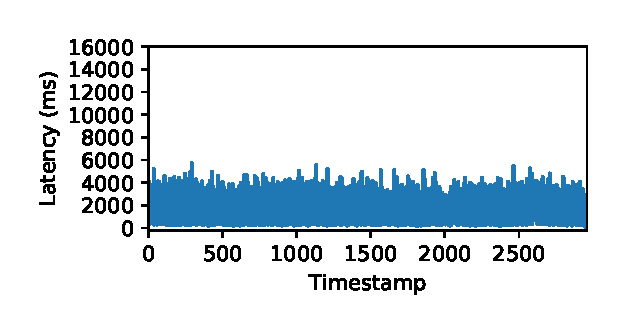
\includegraphics[width=\textwidth]{eps/storm_agg_2node_th_max_ts}

        \caption{2 Node latency with max throughput}
    \end{subfigure}
    ~ 
    \begin{subfigure}[b]{0.3\textwidth}
        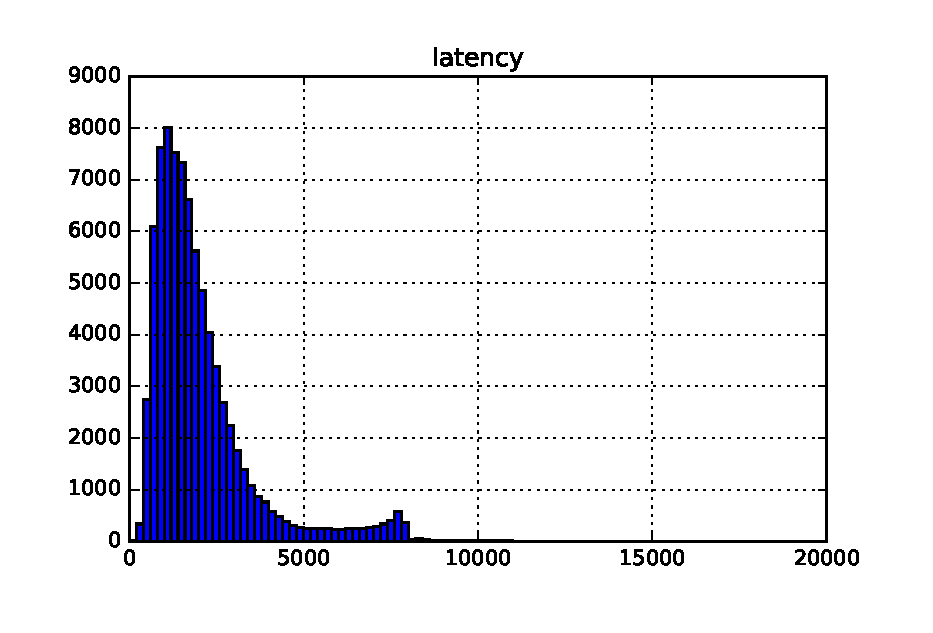
\includegraphics[width=\textwidth]{eps/storm_agg_4node_th_max_hist}
         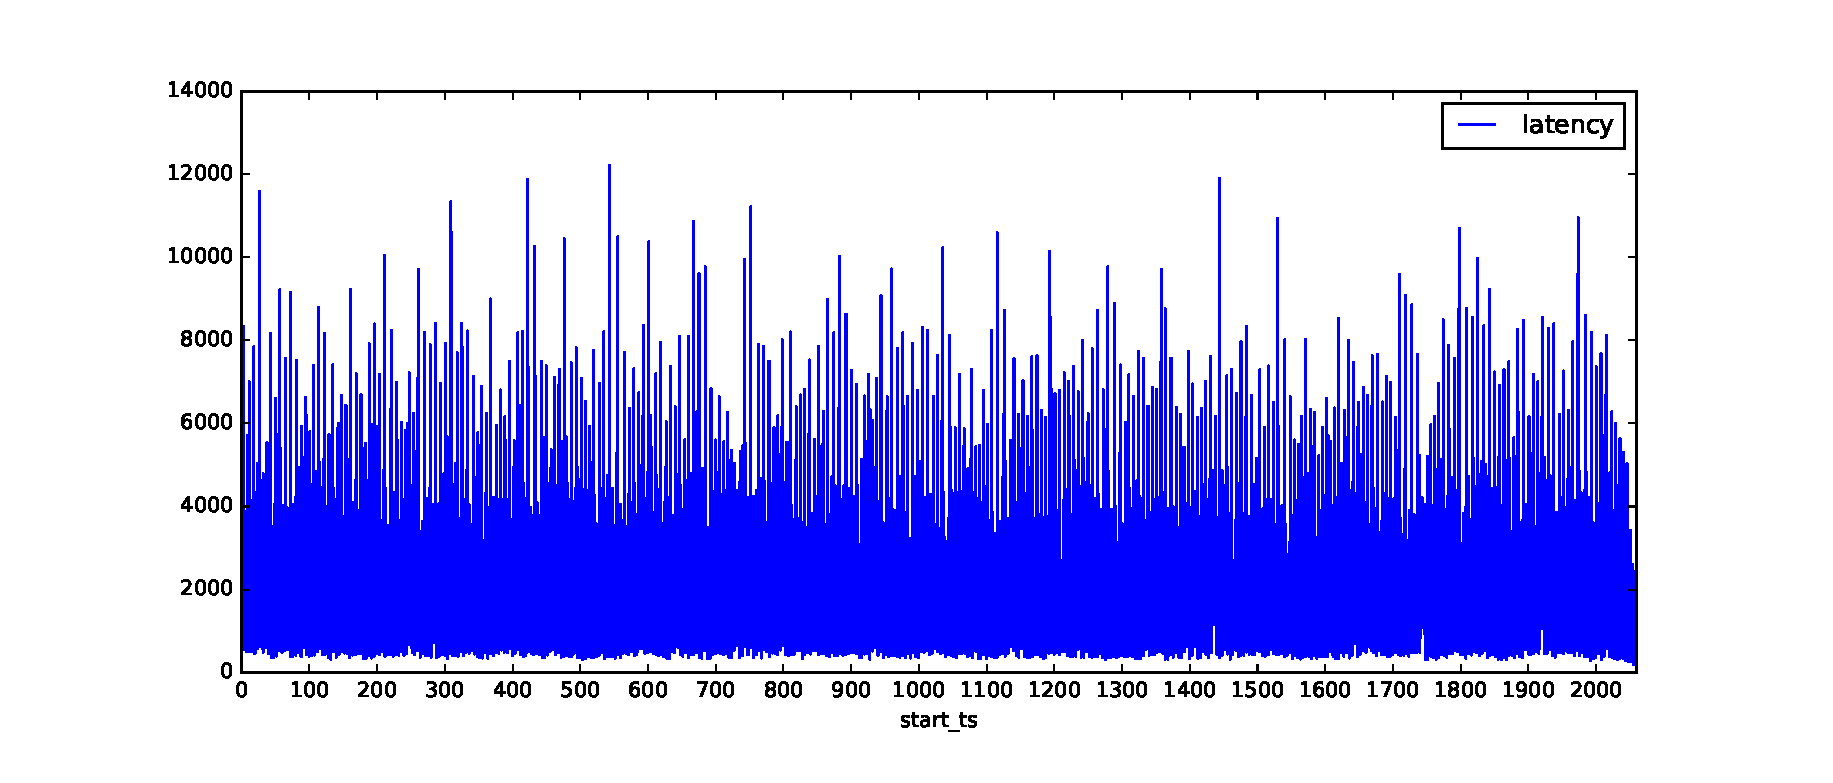
\includegraphics[width=\textwidth]{eps/storm_agg_4node_th_max_ts}

        \caption{4 Node latency with max throughput }
    \end{subfigure}
    ~ 
    \begin{subfigure}[b]{0.3\textwidth}
        \includegraphics[width=\textwidth]{eps/storm_agg_8node_th_max_hist}
         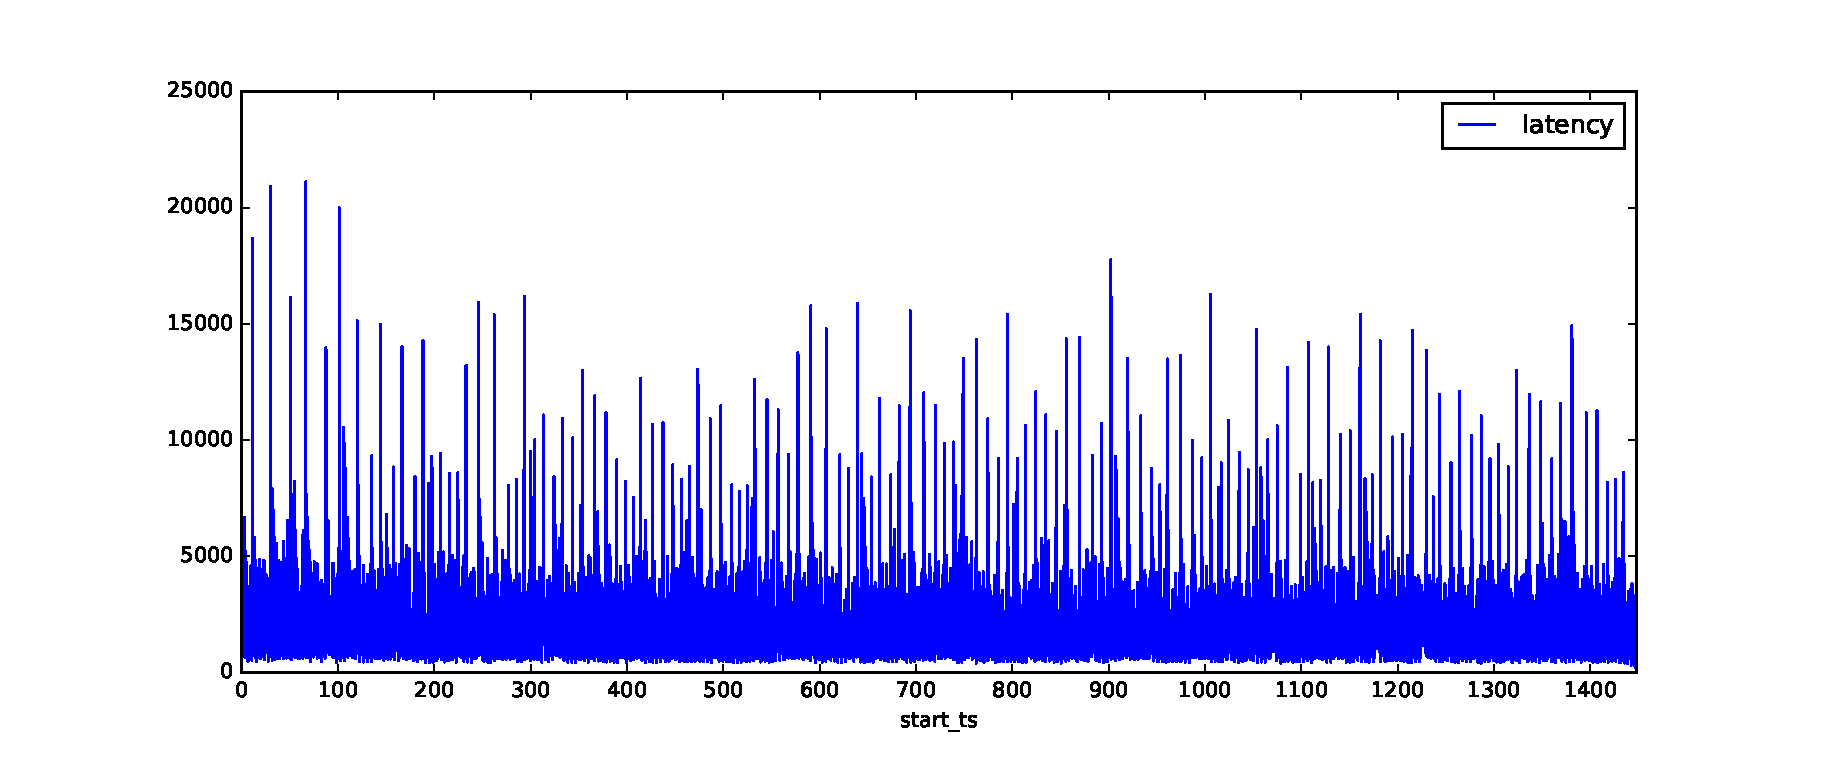
\includegraphics[width=\textwidth]{eps/storm_agg_8node_th_max_ts}

        \caption{8 Node latency with max throughput }
    \end{subfigure}




    \begin{subfigure}[b]{0.3\textwidth}
        \includegraphics[width=\textwidth]{eps/storm_agg_2node_th_90_hist}
         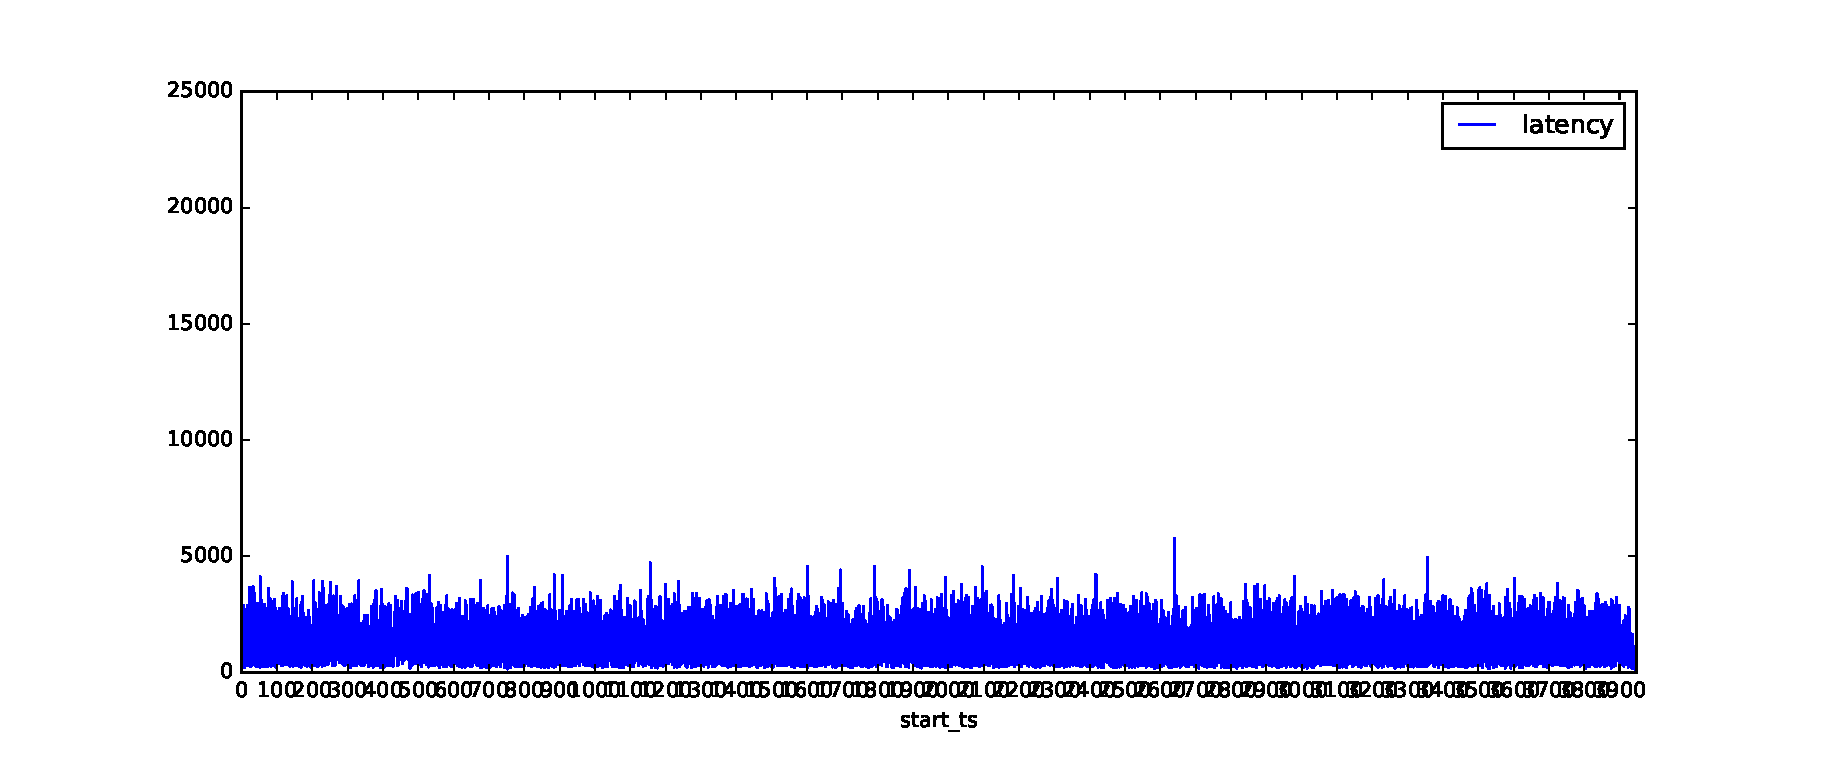
\includegraphics[width=\textwidth]{eps/storm_agg_2node_th_90_ts}

        \caption{2 Node latency with 90\% throughput }
    \end{subfigure}
    ~ 
    \begin{subfigure}[b]{0.3\textwidth}
        \includegraphics[width=\textwidth]{eps/storm_agg_4node_th_90_hist}
         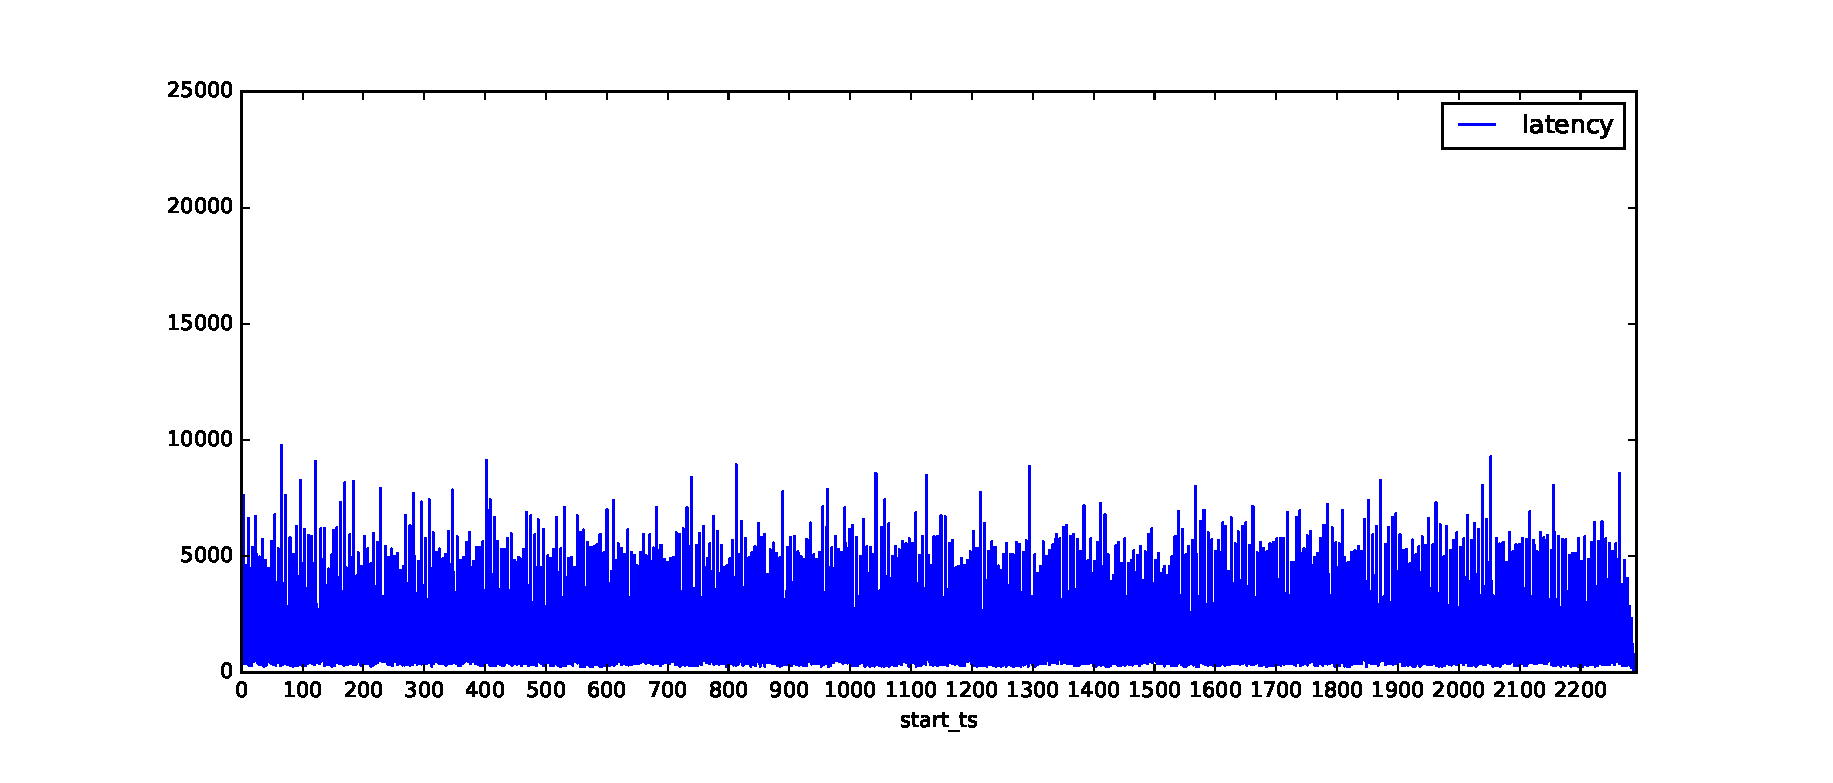
\includegraphics[width=\textwidth]{eps/storm_agg_4node_th_90_ts}

        \caption{4 Node latency with 90\% throughput }
    \end{subfigure}
    ~ 
    \begin{subfigure}[b]{0.3\textwidth}
        \includegraphics[width=\textwidth]{eps/storm_agg_8node_th_90_hist}
         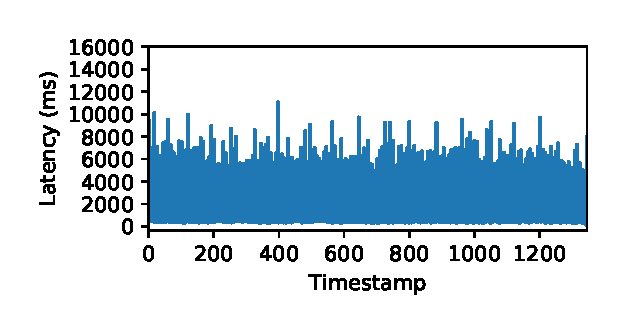
\includegraphics[width=\textwidth]{eps/storm_agg_8node_th_90_ts}

        \caption{4 Node latency with 90\% throughput }
    \end{subfigure}




        \caption{Latency of windowed aggregations for Storm}
\end{figure*}




\subsubsection{Spark}


\include{images/tex/spark_agg}




\subsubsection{Flink}

\begin{figure*}
    \centering
    \begin{subfigure}[b]{0.3\textwidth}
        \includegraphics[width=\textwidth]{eps/flink_agg_2node_th_max_hist}
         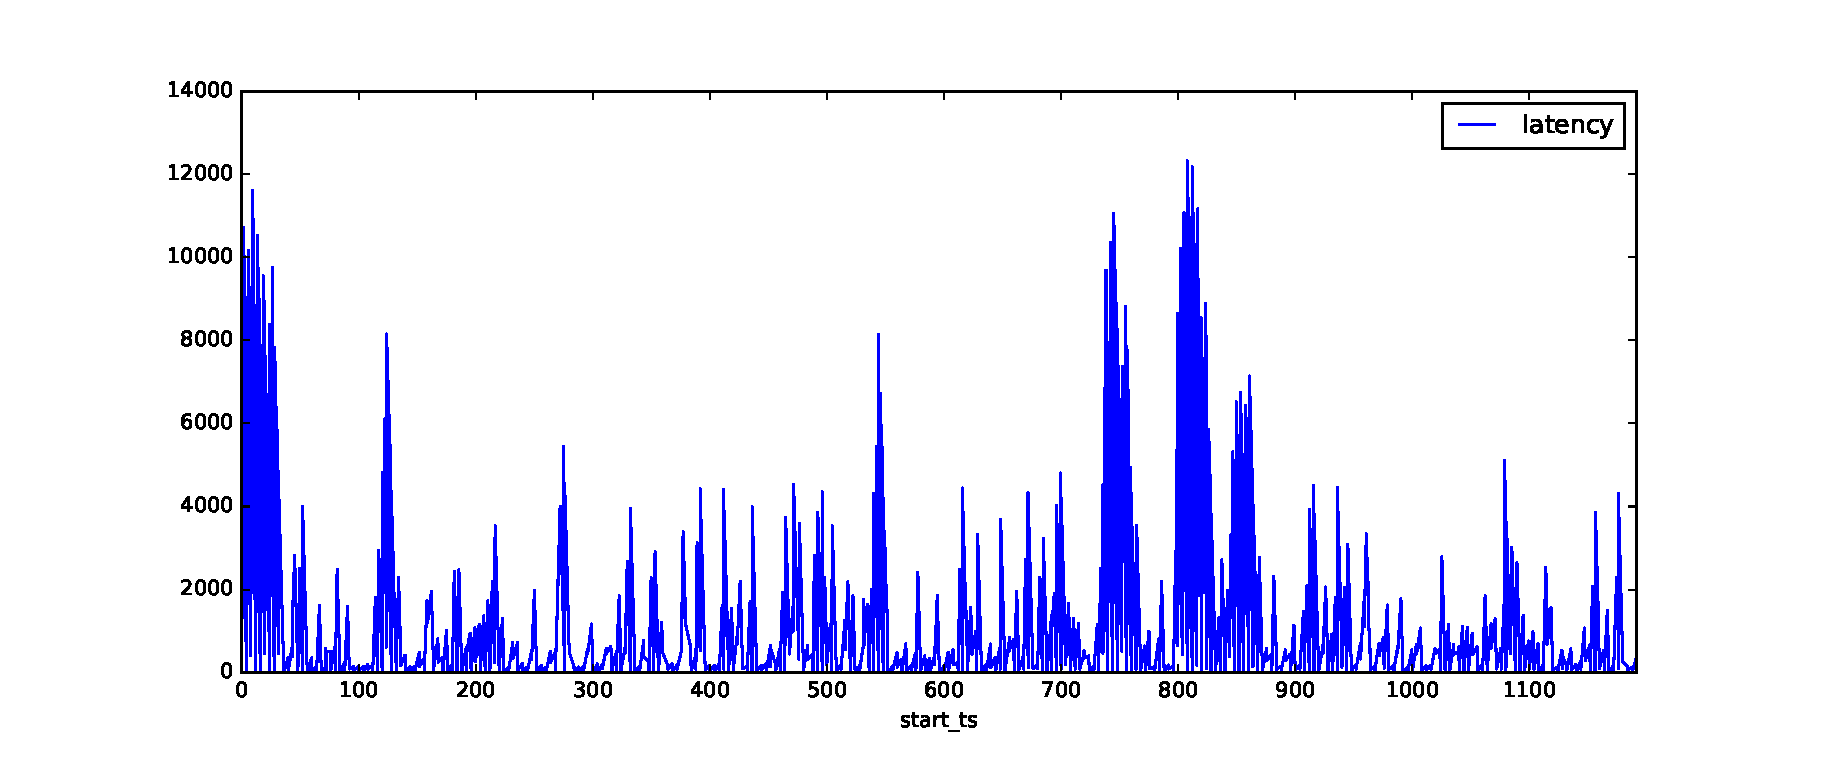
\includegraphics[width=\textwidth]{eps/flink_agg_2node_th_max_ts}

        \caption{2 Node latency with maximum throughput}
    \end{subfigure}
    ~ 
    \begin{subfigure}[b]{0.3\textwidth}
        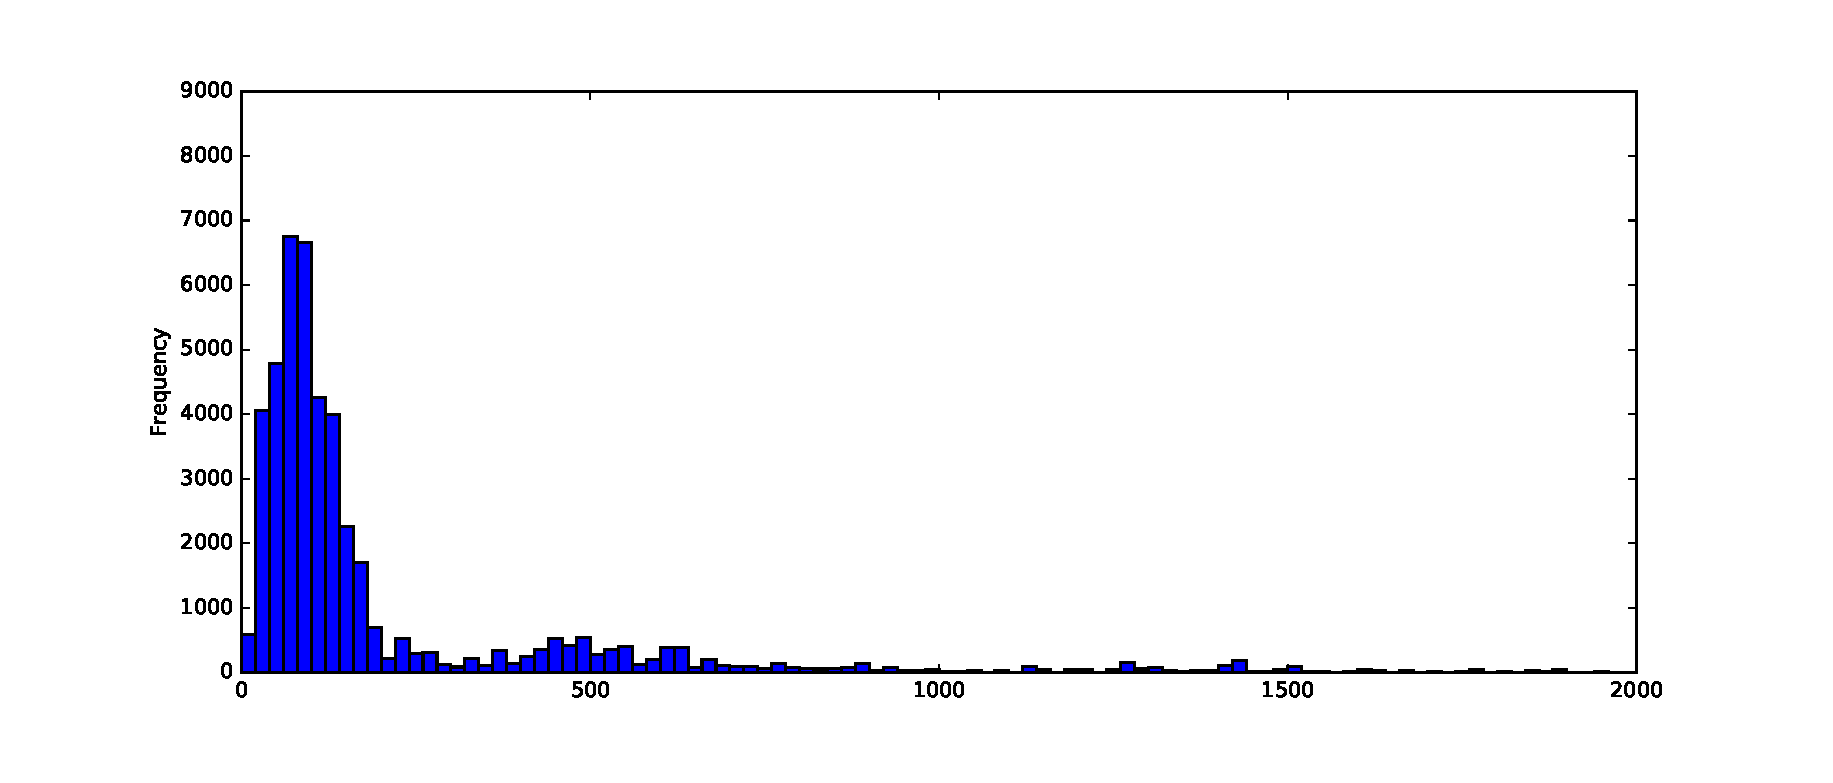
\includegraphics[width=\textwidth]{eps/flink_agg_4node_th_max_hist}
         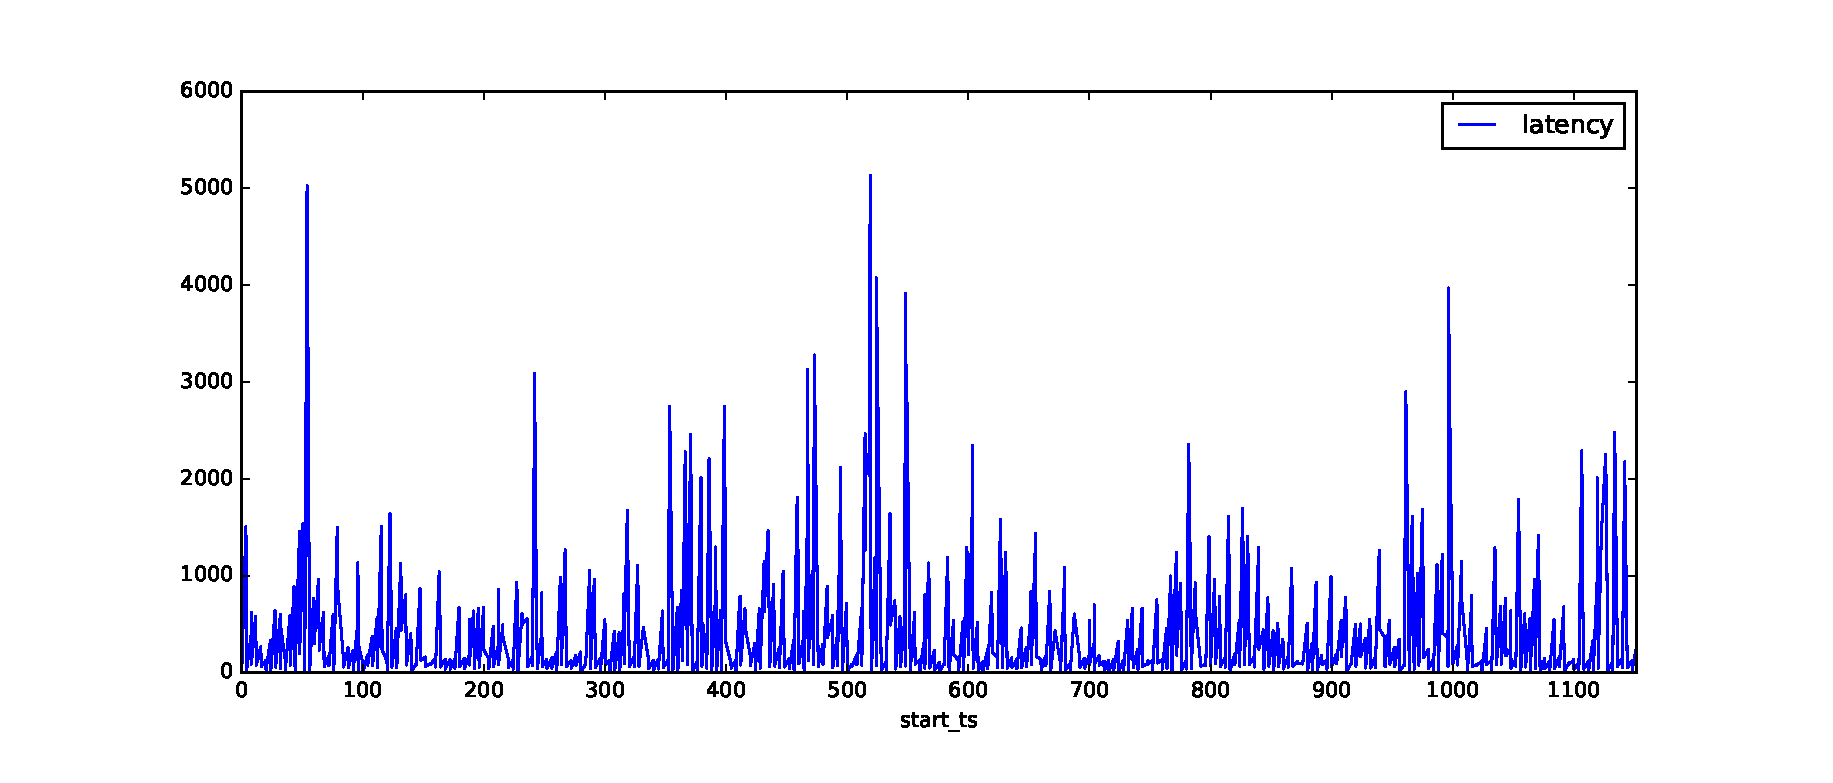
\includegraphics[width=\textwidth]{eps/flink_agg_4node_th_max_ts}

        \caption{4 Node latency with network bounded throughput }
    \end{subfigure}
   ~
    \begin{subfigure}[b]{0.3\textwidth}
        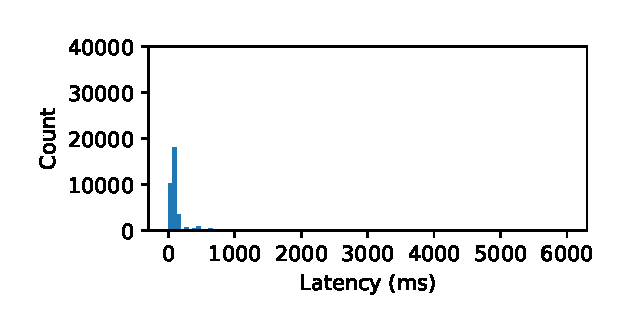
\includegraphics[width=\textwidth]{eps/flink_agg_8node_th_max_hist}
         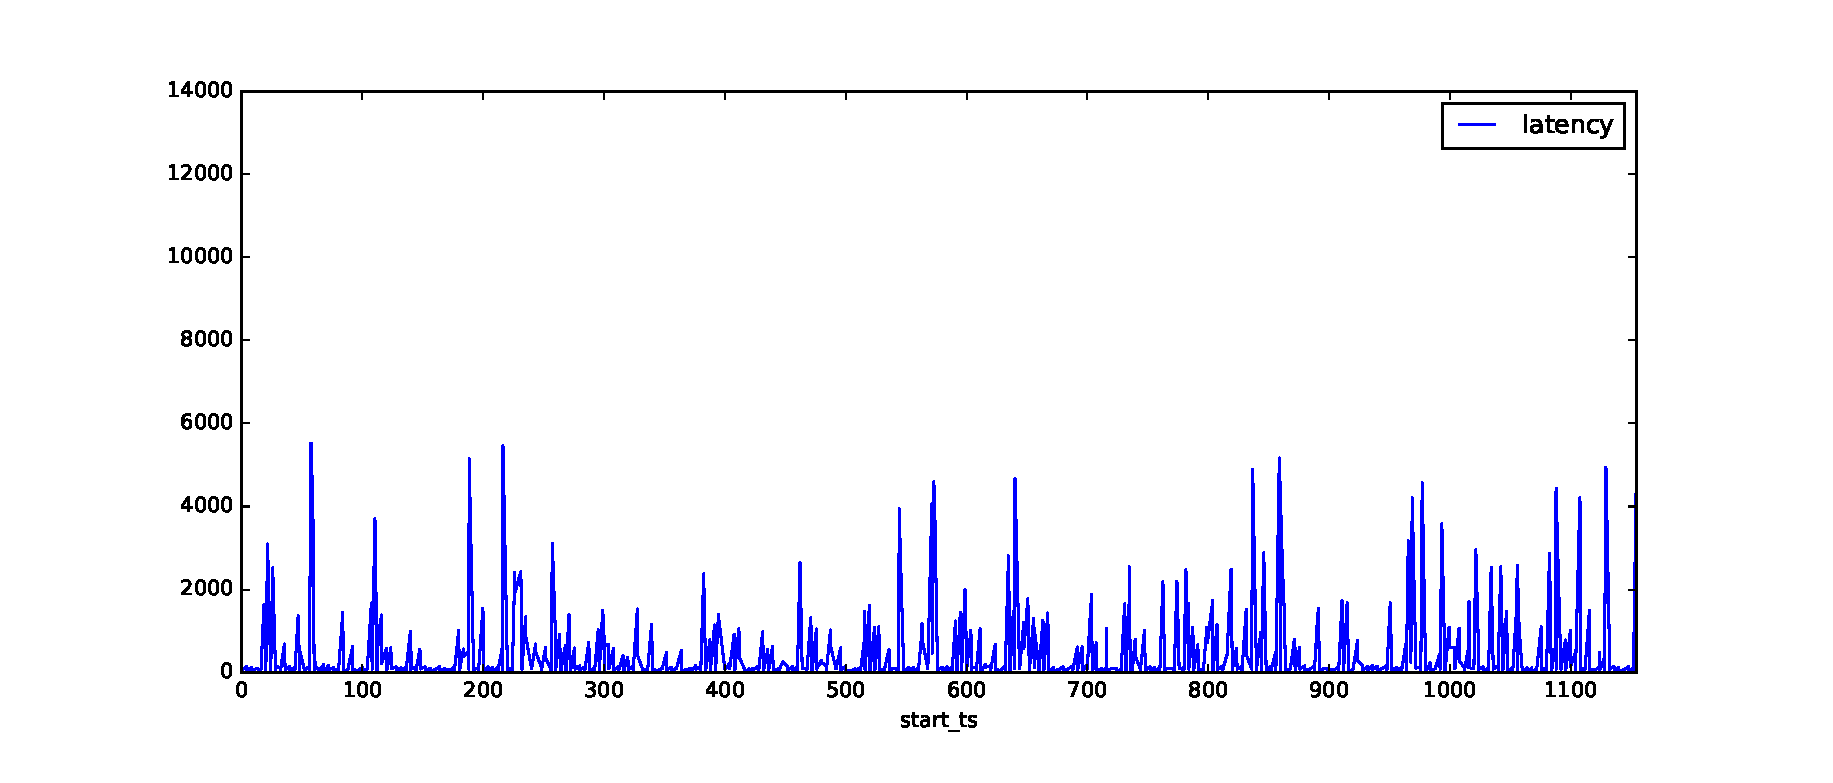
\includegraphics[width=\textwidth]{eps/flink_agg_8node_th_max_ts}

        \caption{8 Node latency with network bounded throughput }
    \end{subfigure}
    ~ 
    \begin{subfigure}[b]{0.3\textwidth}
        \includegraphics[width=\textwidth]{eps/flink_agg_2node_th_90_hist}
         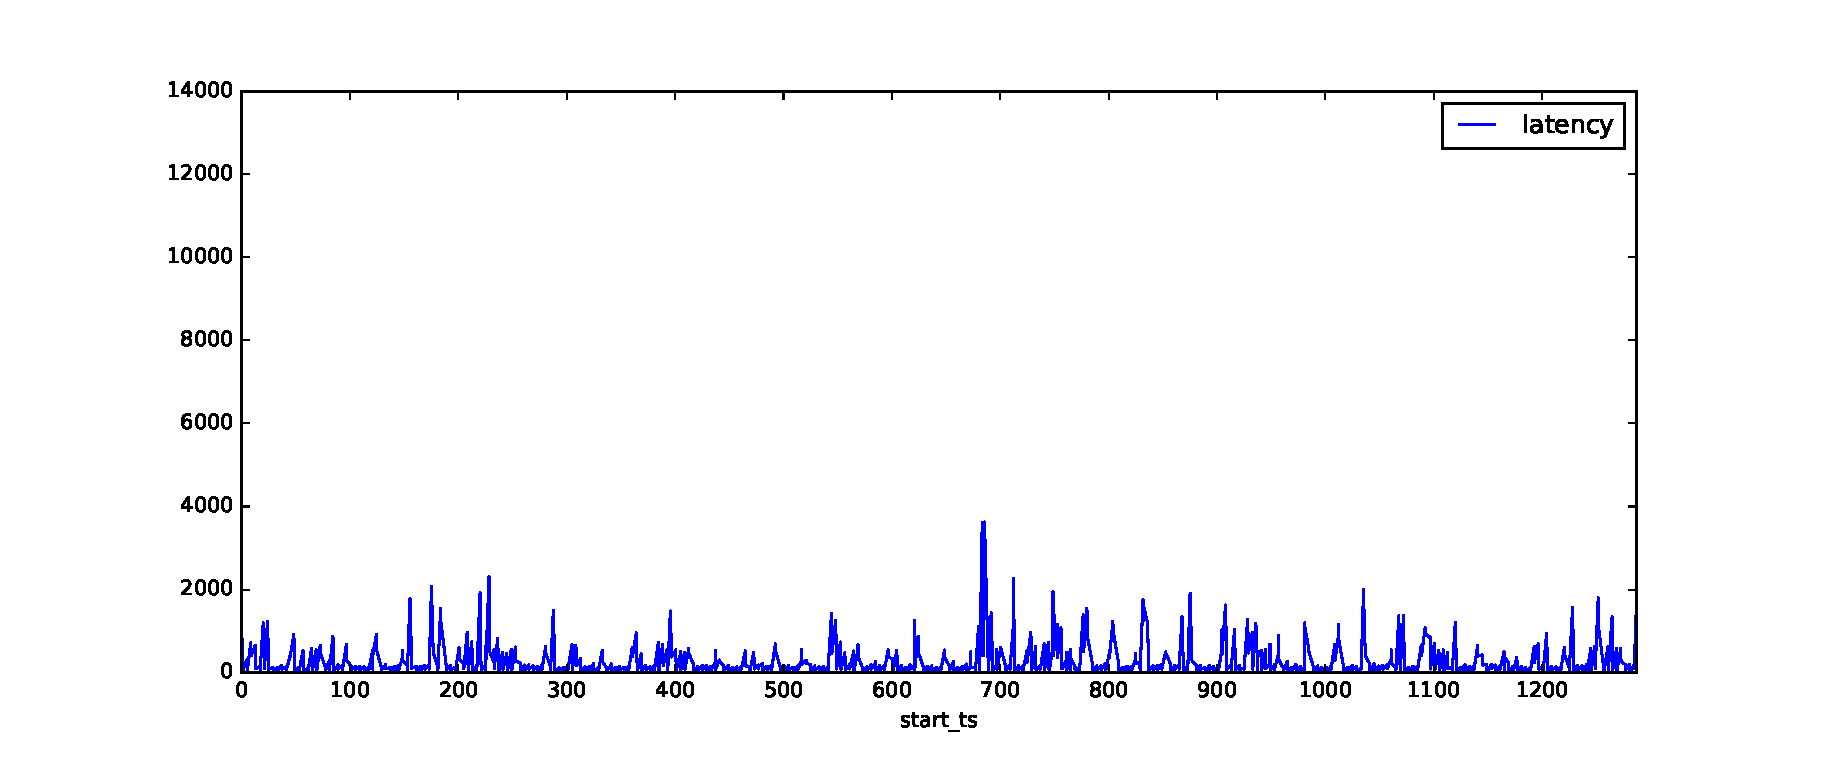
\includegraphics[width=\textwidth]{eps/flink_agg_2node_th_90_ts}

        \caption{2 Node latency with 90\% throughput }
    \end{subfigure}
    ~ 
    \begin{subfigure}[b]{0.3\textwidth}
        \includegraphics[width=\textwidth]{eps/flink_agg_4node_th_90_hist}
         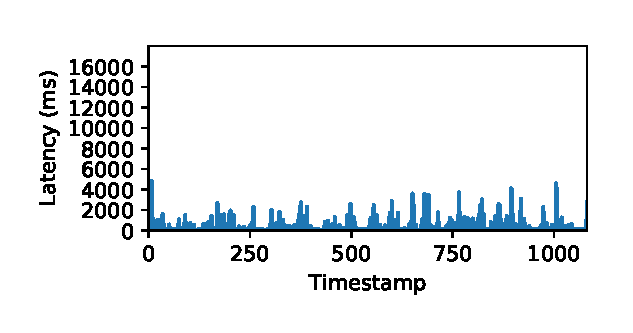
\includegraphics[width=\textwidth]{eps/flink_agg_4node_th_90_ts}

        \caption{2 Node latency with 90\% throughput }
    \end{subfigure}
    ~ 
    \begin{subfigure}[b]{0.3\textwidth}
        \includegraphics[width=\textwidth]{eps/flink_agg_8node_th_90_hist}
         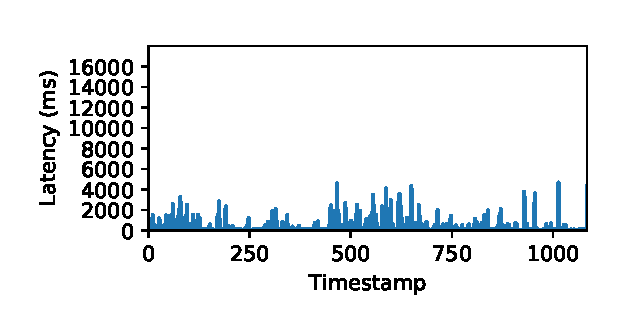
\includegraphics[width=\textwidth]{eps/flink_agg_8node_th_90_ts}

        \caption{2 Node latency with 90\% throughput }
    \end{subfigure}




        \caption{Latency of windowed aggregations for Flink}
\end{figure*}




\subsection{Joins}

\subsubsection{Storm}

\subsubsection{Spark}

\include{images/tex/spark_join}

\subsubsection{Flink}

\include{images/tex/flink_join}




